% Chapter Template

\chapter{Data gathering and preprocessing} % Main chapter title

\label{Chapter2} % Change X to a consecutive number; for referencing this chapter elsewhere, use \ref{ChapterX}

%----------------------------------------------------------------------------------------
%	SECTION 1
%----------------------------------------------------------------------------------------

Data was sourced from several streams. Veðurstofan provided recordings from weather stations all around the Iceland. Data was downloaded from Copernicus Arctic Regional Reanalysis dataset (CARRA). A land elevation model was also provided by Veðurstofan.

\section{Automatic Weather Station Data}

Veðurstofan provided recordings from 412 weather stations all around Iceland. The location of these weather stations can be seen in Figure \ref{fig:aws_map}. These automatic weather stations (AWS) are at a height of 10 meters above ground level. The information that is provided by these AWS is presented in two different type of documents, hourly and 10 minute documents. The hourly documents are summations of the 10 minute documents, with the exception that any errors (so called nails) still in the 10 minute documents should have been removed from the hourly documents. Each type of document contain the following information: the date and time, the station number (that can be converted to the coordinates using another document), the average wind speed, the wind gust, the standard deviation of the wind gust, the direction of the wind and the standard deviation for the wind direction. These features for each of the stations go back at least two decades, but do not have the same start date. This thesis does not look at the data as a time series, it tries to make predictions using only the information at a given point in time.

\begin{figure}[h]
    \caption{Locations of Automatic Weather Stations in Iceland}
    \label{fig:aws_map}
    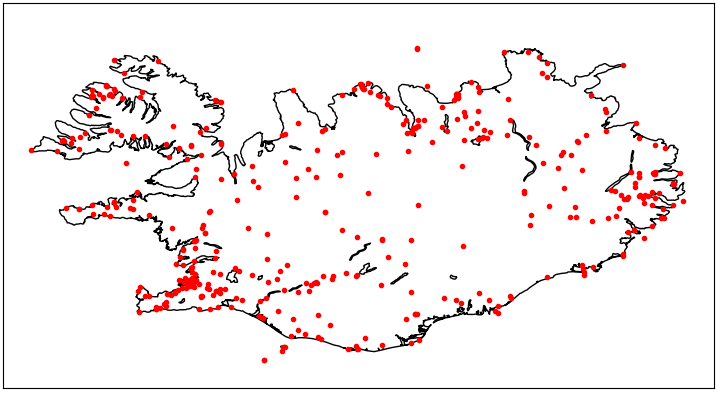
\includegraphics[scale = 0.75]{Figures/weather_stations.png}
\end{figure}

\section{Carra Data}
The CARRA dataset goes back to September 1990 and is currently updated monthly, with a latency of 2-3 months. The oldest Vedurstofu data example that fulfills given criteria is from \startDateVedur. This is covered by Carra. A few of the newer points from AWS were not available from Carra when data was gathered. The Carra dataset is available for two regions, west and east. Each of these covers a vastly larger area than the area of interest. It is possible to request a subsection of the area, a rectangular subsection of the area. This leads to having to store a large amount of data, because it is not possible to ask for specific points of interest. To get the data one has two options. Their web interface or using their API client. Using the API client is the only realistic option here, as there were thousands of requests made for different times.

Each request is made by going through all instances of the Veðurstofu data were able to fulfill the requirements (of mean wind speed reaching \averageWindSpeedLimit m/s over a 10 minute interval). For each such observation in the Veðurstofa data, two API calls excluding redundancy are needed. One for the 3 hour interval before and one for the 3 hour interval after, if the data point doesn't fall exactly one of the three hour interval times. That is if the observation was at 13:00, Carra data for noon and 15:00 would have to be queried. Date and times were generated automatically from the AWS and requested by calling the client. Using these datapoints, interpolation was used to get an estimation for the point of the given weather station. The Carra data contains several types of layers. These are single levels, model levels, height levels, pressure levels. The data for this observation was downloaded from height levels. That is, data was requested at heights of 15, 150, 250 and 500 meters above ground. For each point 4 parameters were requested, wind speed, wind direction, pressure and temperature. Each of these features needed to be interpolated to create data for model to be trained on.

After using this method to request terabytes of data, it was discovered that it is apparently possible to query a specific area. This decreased the size of each file created after a request from around 50 MB to around 2 MB. Downloading and processing this data would take a lot less time. The bottleneck for retrieving the data is the request time. That is the time the request is queued and running (server preparing the data) before it begins downloading. This could range from almost immediate to 30 minutes. This problem was exacerbated by the fact that the climate data store (CDS) was undergoing updates during the winter and spring of 2023/2024, which increased the wait time and sometimes resulted in queries not being responded to. This meant that the time it would take to retrieve the remaining information went from around a day, when the requests were at their quickest, to many months, something that would not be possible given the time frame of the project. Fortunately these problems were only particularly time consuming during mid winter.

\section{Elevation data}
Veðurstofa provided a tif file containing the elevation of Iceland on a 20 meter by 20 meter grid. This file encompasses Iceland and is around 685 Mb. A good amount of time was spent finding a data structure that was best for lookup when trying to find points within a certain area. The country was divided into 10 parts (as only around 13\% of the file was able to be read into memory at each time as a part of dictionary object) with boundary boxes. A quadtree was constructed for each of the sections, so as to simplify the lookup. A quadtree allows for efficient lookup by searching for points that intersect a given boundary. A quadtree, like the name indicates, is a tree structure. To initialize it a boundary box is given. This boundary box is then the parent of exactly four nodes and so on, dividing the area in four at each level and allowing quick lookup. This was not necessary as the Python package Rasterio allowed for quick lookup with it's index and the affine transform. Using this package it is possible to quickly look up elevation given coordinates using matrix calculations.